\documentclass{article}

%================  CUSTOMIZATION  =================================================%

\usepackage{../KjelsethReportStyle}

%================  METADATA  ======================================================%

\title{\fontsize{24}{36}\selectfont Elektroniske enheter og kretser\\ % Input title
Lab 01} % Line 2 of title, \\ means next line.

\author{{\ttfamily Sølve Kjelseth}} % Input your name.
% replace \ttfamily with \normalfont to make it regular font.
% (removing \ttfamily will not do this automatically.

\date{\today} % Auto updates the date, untill you export it.


%================  START OF DOCUMENT  =============================================%

\begin{document}

\maketitle % Makes title front page based on the title, author and date metadata, change at the top

%================  SECTION  =======================================================%

\addtocontents{toc}{\protect\setcounter{tocdepth}{0}} % Temporarily hide from TOC
\section{Introduction} % Numbered section named Introduction
This is the first report in this course, detailing the completion of the first lab exercise.\par
\vfill
Note: As always, the \LaTeX\ file and all other assets, such as text, images, graphs and code made by me for this project is open source with the MIT licence, see
\linkgithub[true][0.5]{my GitHub}

\clearpage

%================  SECTION  =======================================================%

\tableofcontents % Generate TOC
\hfill
\listoffigures % List of figures
\hfill
\listoftables % List of tables
\addtocontents{toc}{\protect\setcounter{tocdepth}{2}} % Restore TOC depth

%================  SECTION  =======================================================%

\section{Part 1 - Diode test}
This Part is about testing a diode charachteristics with a multimeter. This means it is inherently not perfect, but it will function as a reference measurment.

%================  SINGLE FIGURE  =================================================%

\begin{figure}[h]
    \centering
    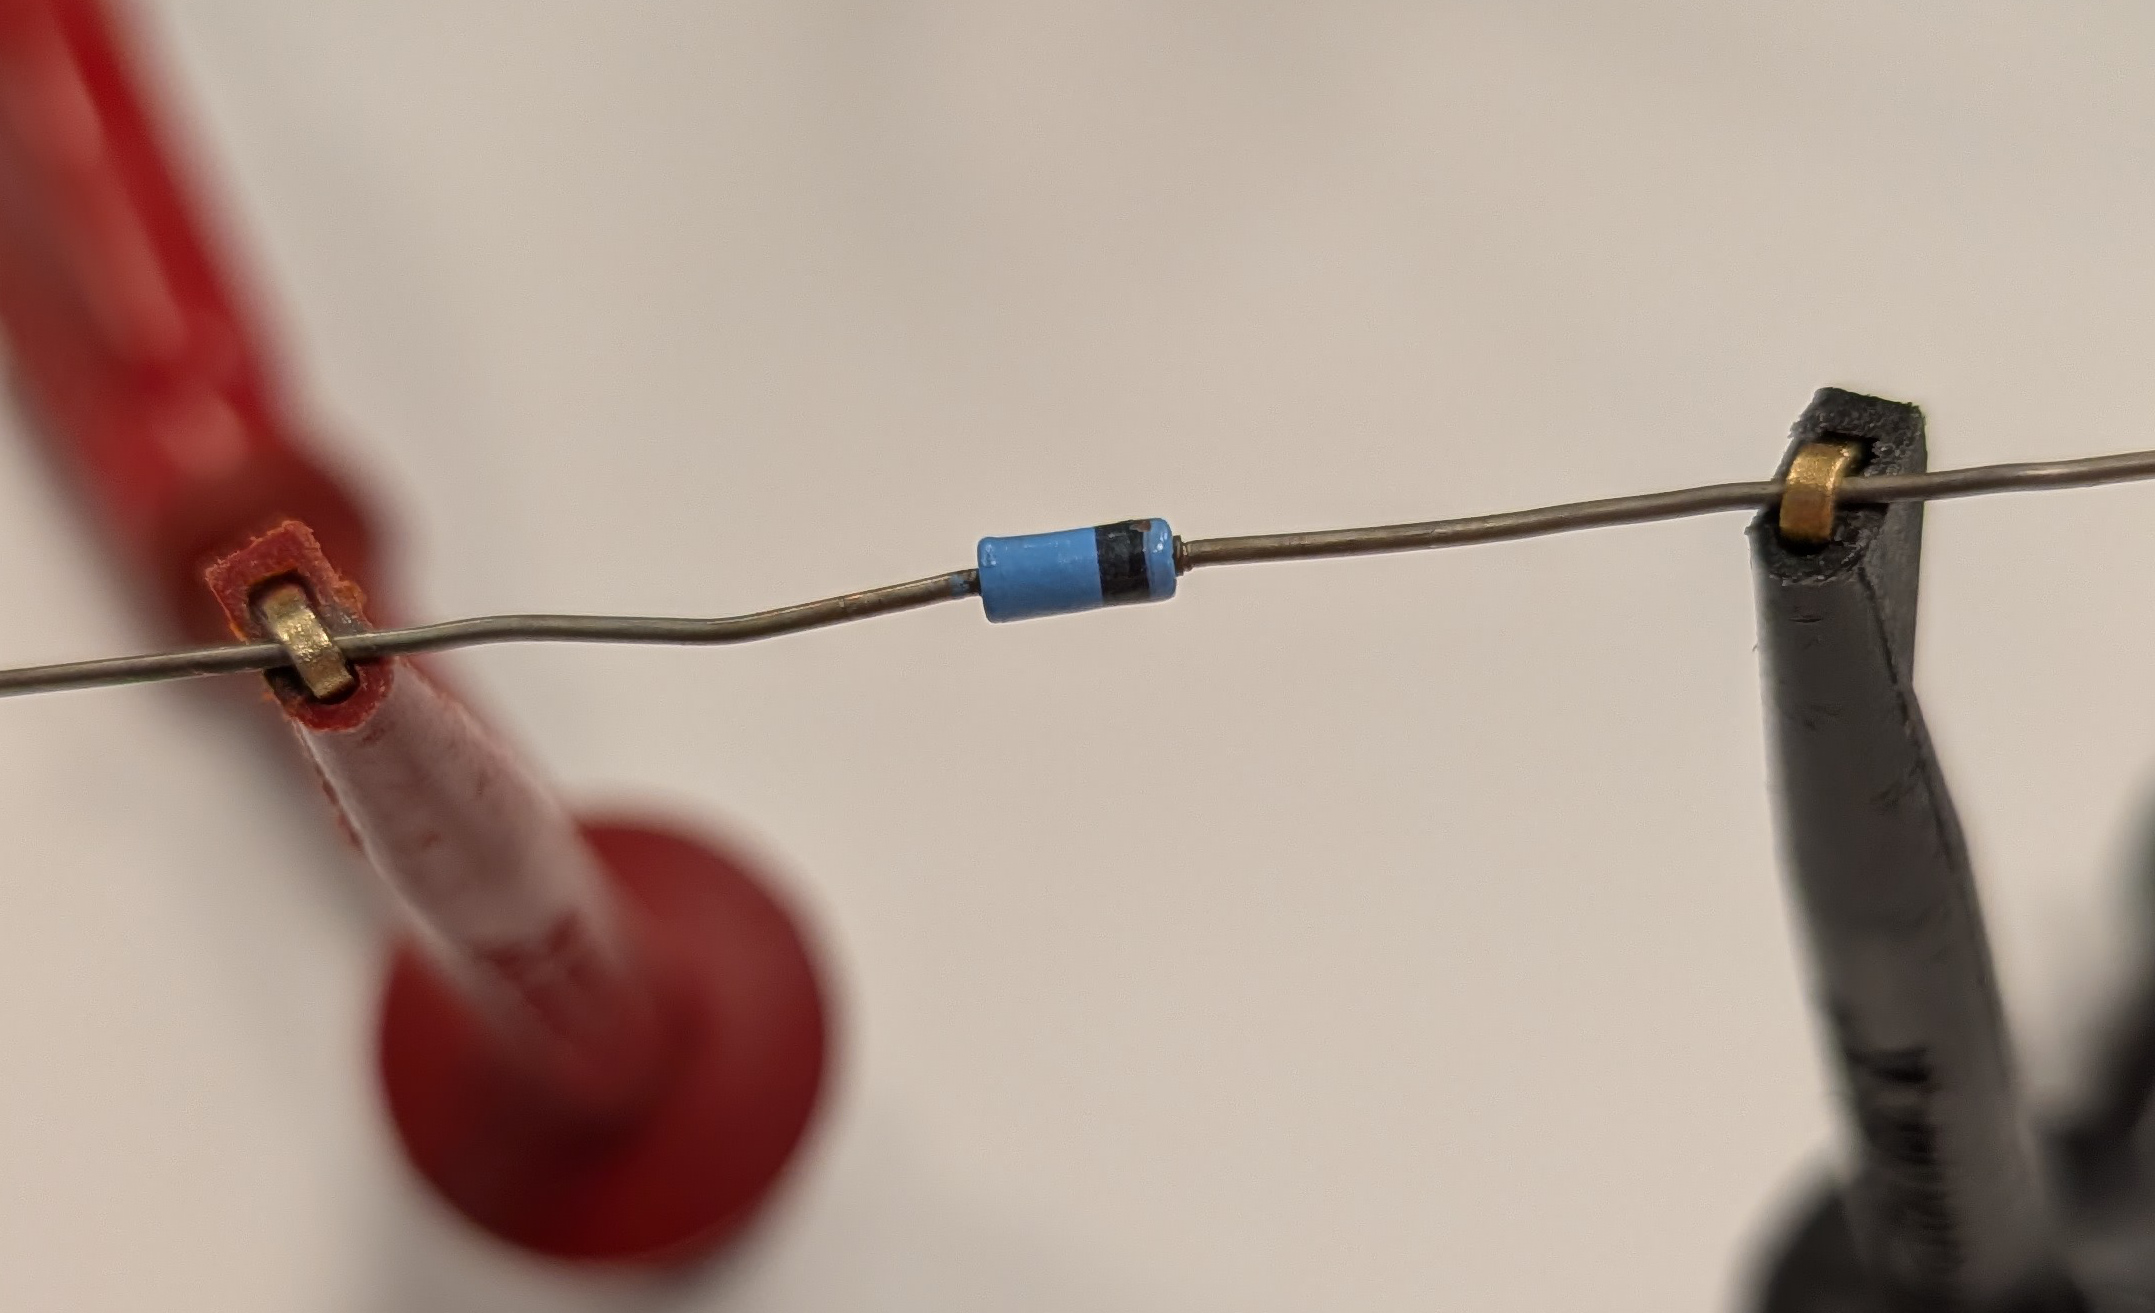
\includegraphics[width=\textwidth]{Part1.jpg}
    \caption{Diode being measured}
    \label{fig:part1}
\end{figure}

%================  TABLE  =========================================================%

% Table generated by Excel2LaTeX from sheet 'Sheet1'
\begin{table}[htbp]
  \centering
  \caption{Diode measurments}
    \begin{tabular}{|l|lr|l|lr|}
    \hline
    Voltage forward & \multicolumn{1}{r}{0.593} & \multicolumn{1}{l|}{V} & Resistance forward & \multicolumn{1}{r}{225400} & \multicolumn{1}{l|}{\Omega} \bigstrut\\
    \hline
    Voltage reverse & OL    &       & Resistance reverse & OL    &  \bigstrut\\
    \hline
    \end{tabular}%
  \label{tab:part1}%
\end{table}%


Interesting to note that the measured resistance in forward-bias of the diode fluctuated a lot. It went into high \(\SI{}{\mega\ohm}\) to low tens of \(\SI{}{\kilo\ohm}\). It was most stable around \(\SI{200}{\kilo\ohm}\) and one of these measurmens was therfore noted down. This could be because the multimeter is acting as a powersupply in resistance measuring mode and depending on the voltage chosen by the autoranging multimeter the diode behaviour differs.

%================  SECTION  =======================================================%

\section{Part 2 - Forward-bias charachteristics}
This Part is about testing the diode charachteristics for forward-bias. The values was stored in a table (RAW data like this is found on the \linkgithub{GitHub}) and then a plot was made to compare the current through the diode \(I_D\) with the voltage drop over the diode \(V_D\).

%================  SINGLE FIGURE  =================================================%

\begin{figure}[h]
    \centering
    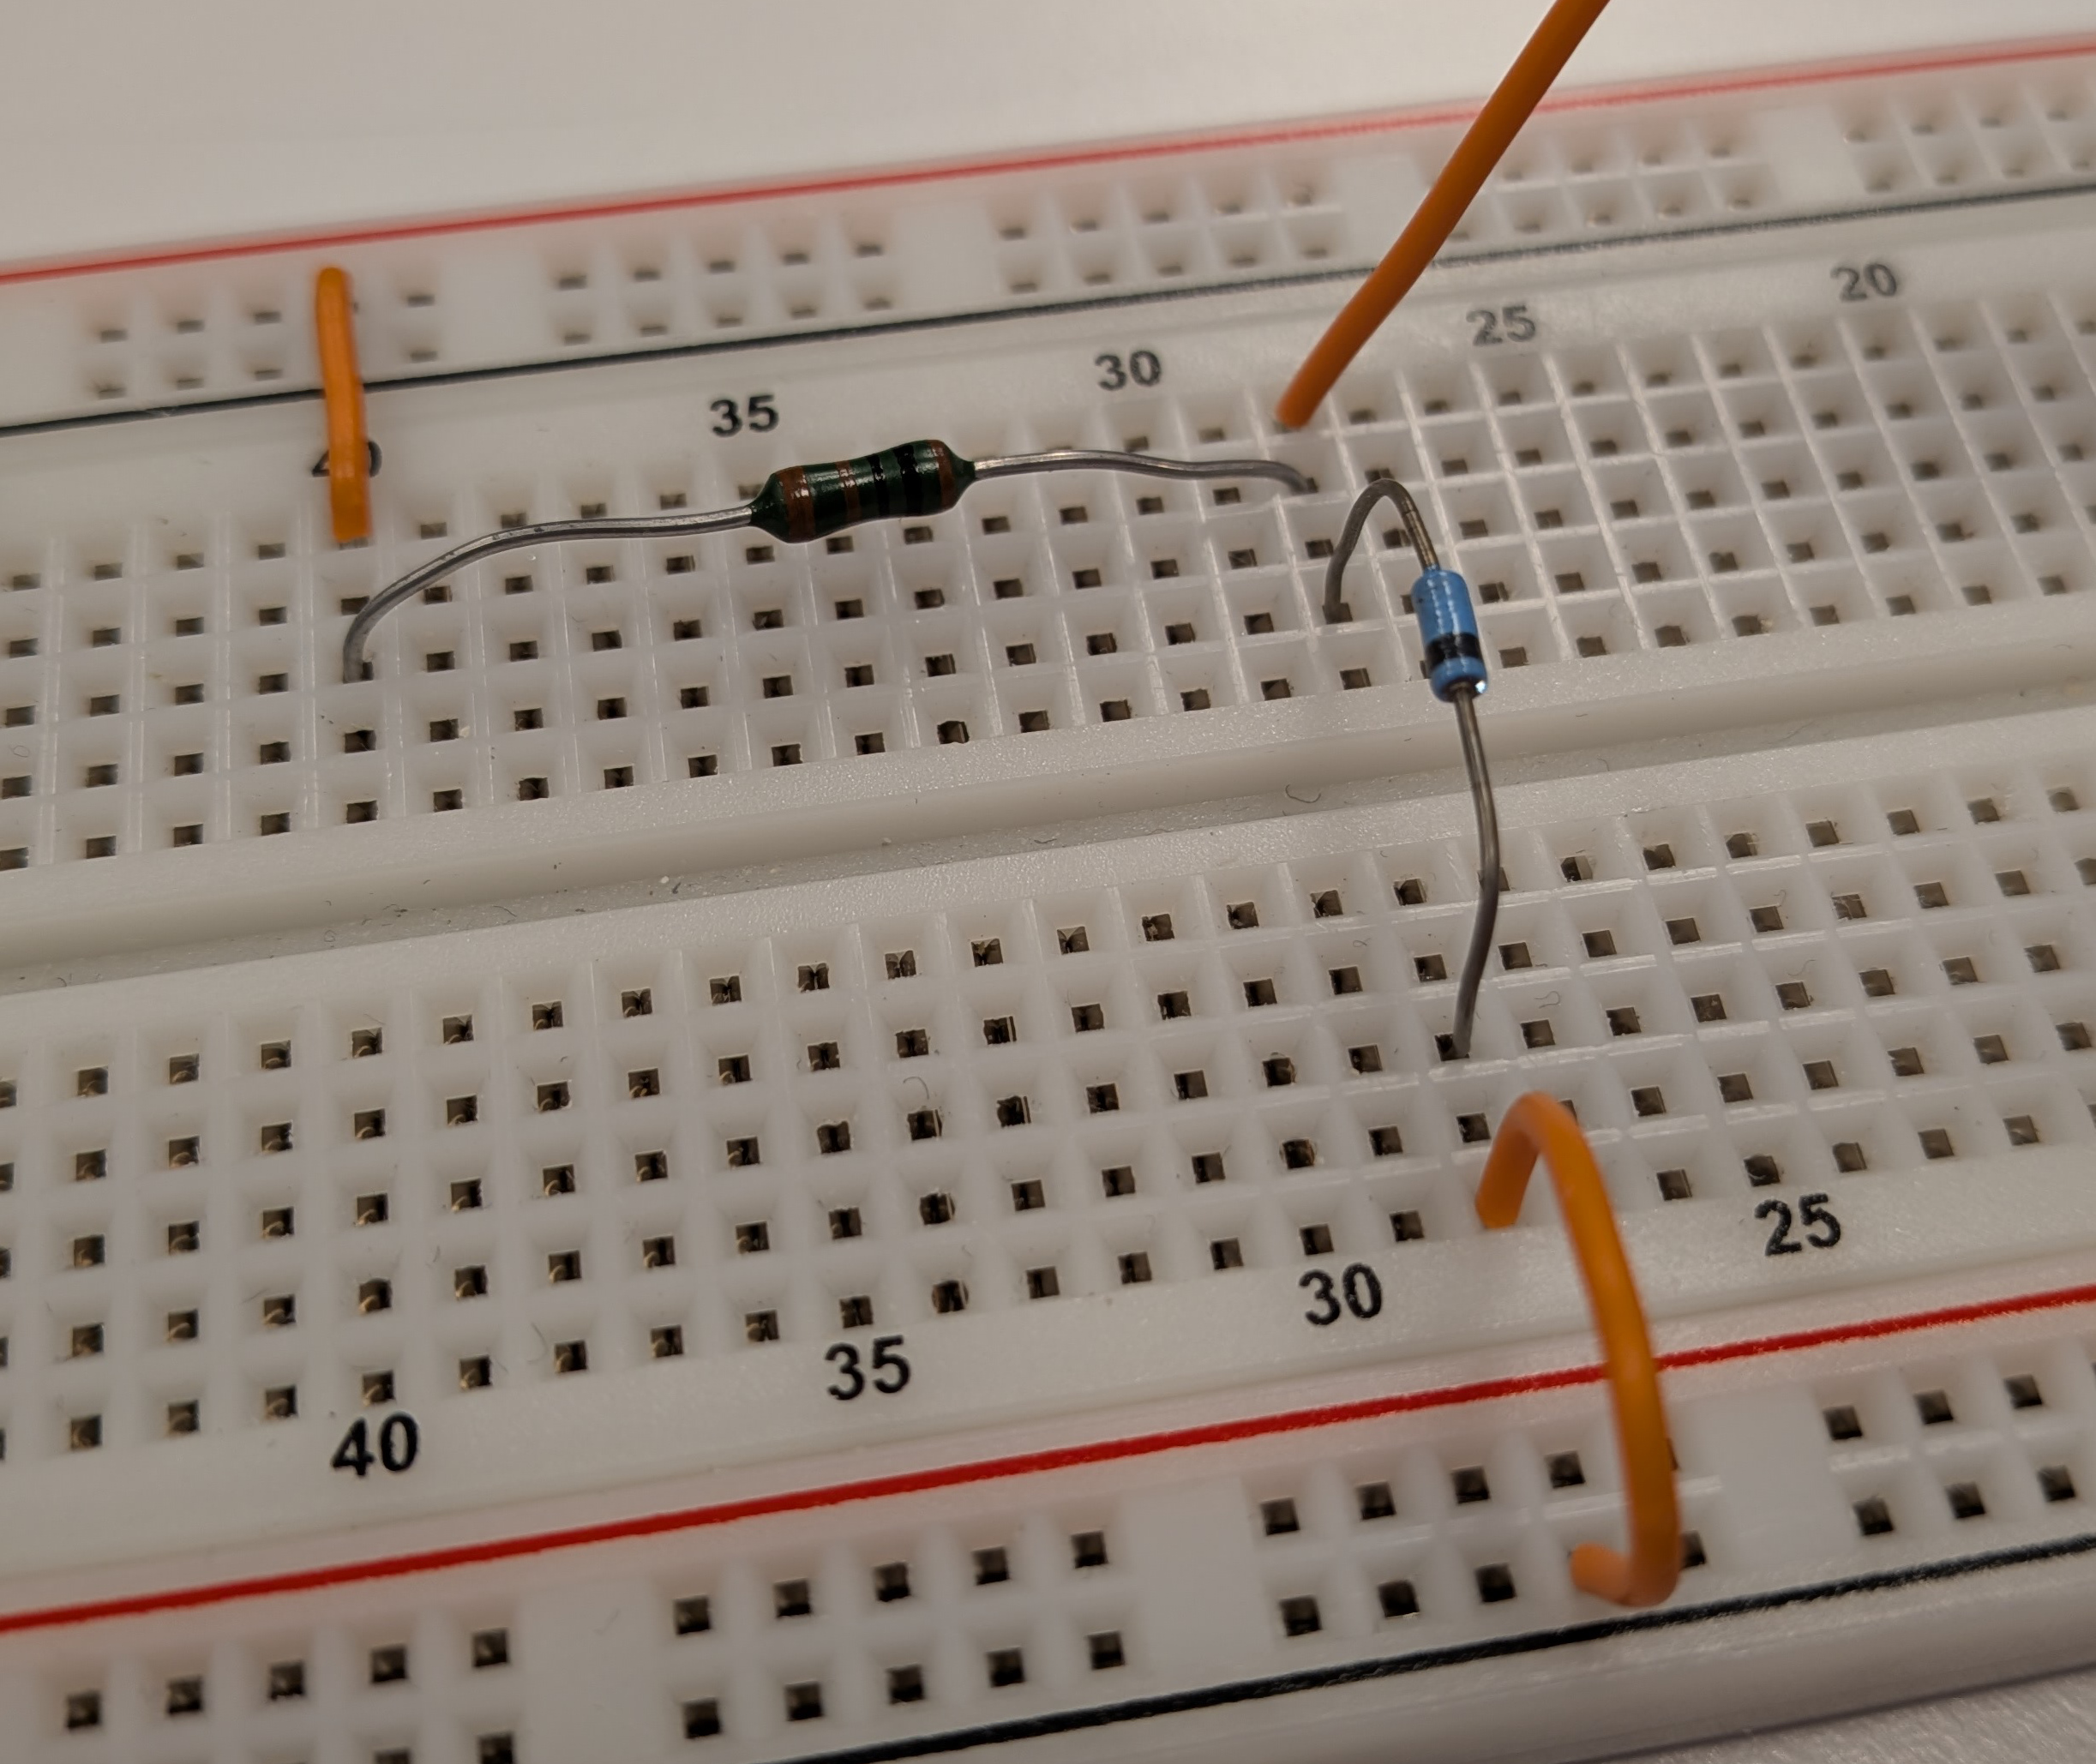
\includegraphics[width=\textwidth]{Part2.jpg}
    \caption{Part 2 circuit}
    \label{fig:Part2}
\end{figure}

\clearpage

%================  SINGLE FIGURE  =================================================%

\begin{figure}[h]
    \centering
    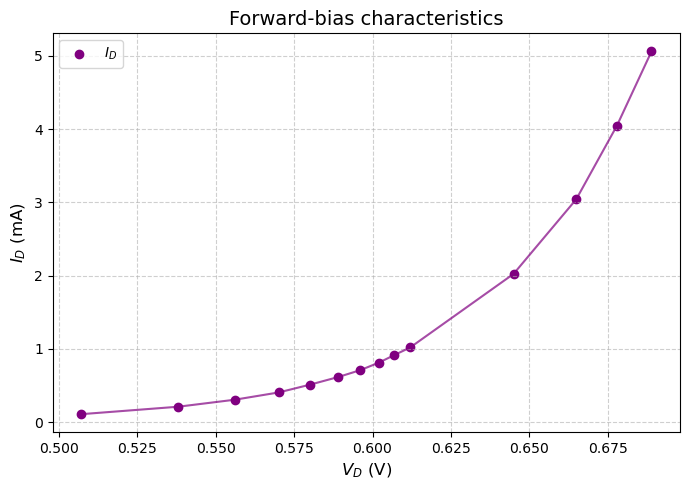
\includegraphics[width=\textwidth]{Part2Plot.png}
    \caption{Plot of forward-bias charachteristics}
    \label{fig:Part2Plot}
\end{figure}

Now when when extending the plot all the way to the origin it gets a charachteristic that looks a lot different. As seen in Figure~\ref{fig:Part2PlotExtended} it looks like after the initial curve the value gets linear.

\clearpage

%================  SINGLE FIGURE  =================================================%

\begin{figure}[h]
    \centering
    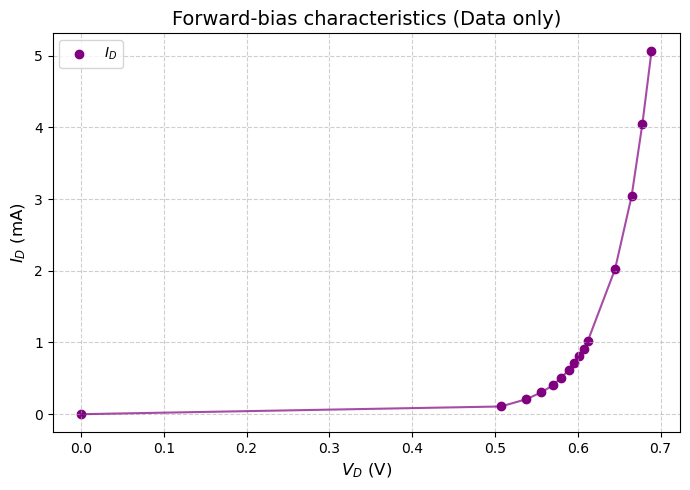
\includegraphics[width=\textwidth]{Part2PlotExtended.png}
    \caption{Extended plot of forward-bias charachteristics}
    \label{fig:Part2PlotExtended}
\end{figure}

%================  SECTION  =======================================================%

\section{Part 3 - Reverse-bias}
This Part is about testing the reverse-bias current. Measurments was made and noted in the table, note that the assumed resistive value of the voltmeter is specified by the assignment.

%================  SINGLE FIGURE  =================================================%

\begin{figure}[h]
    \centering
    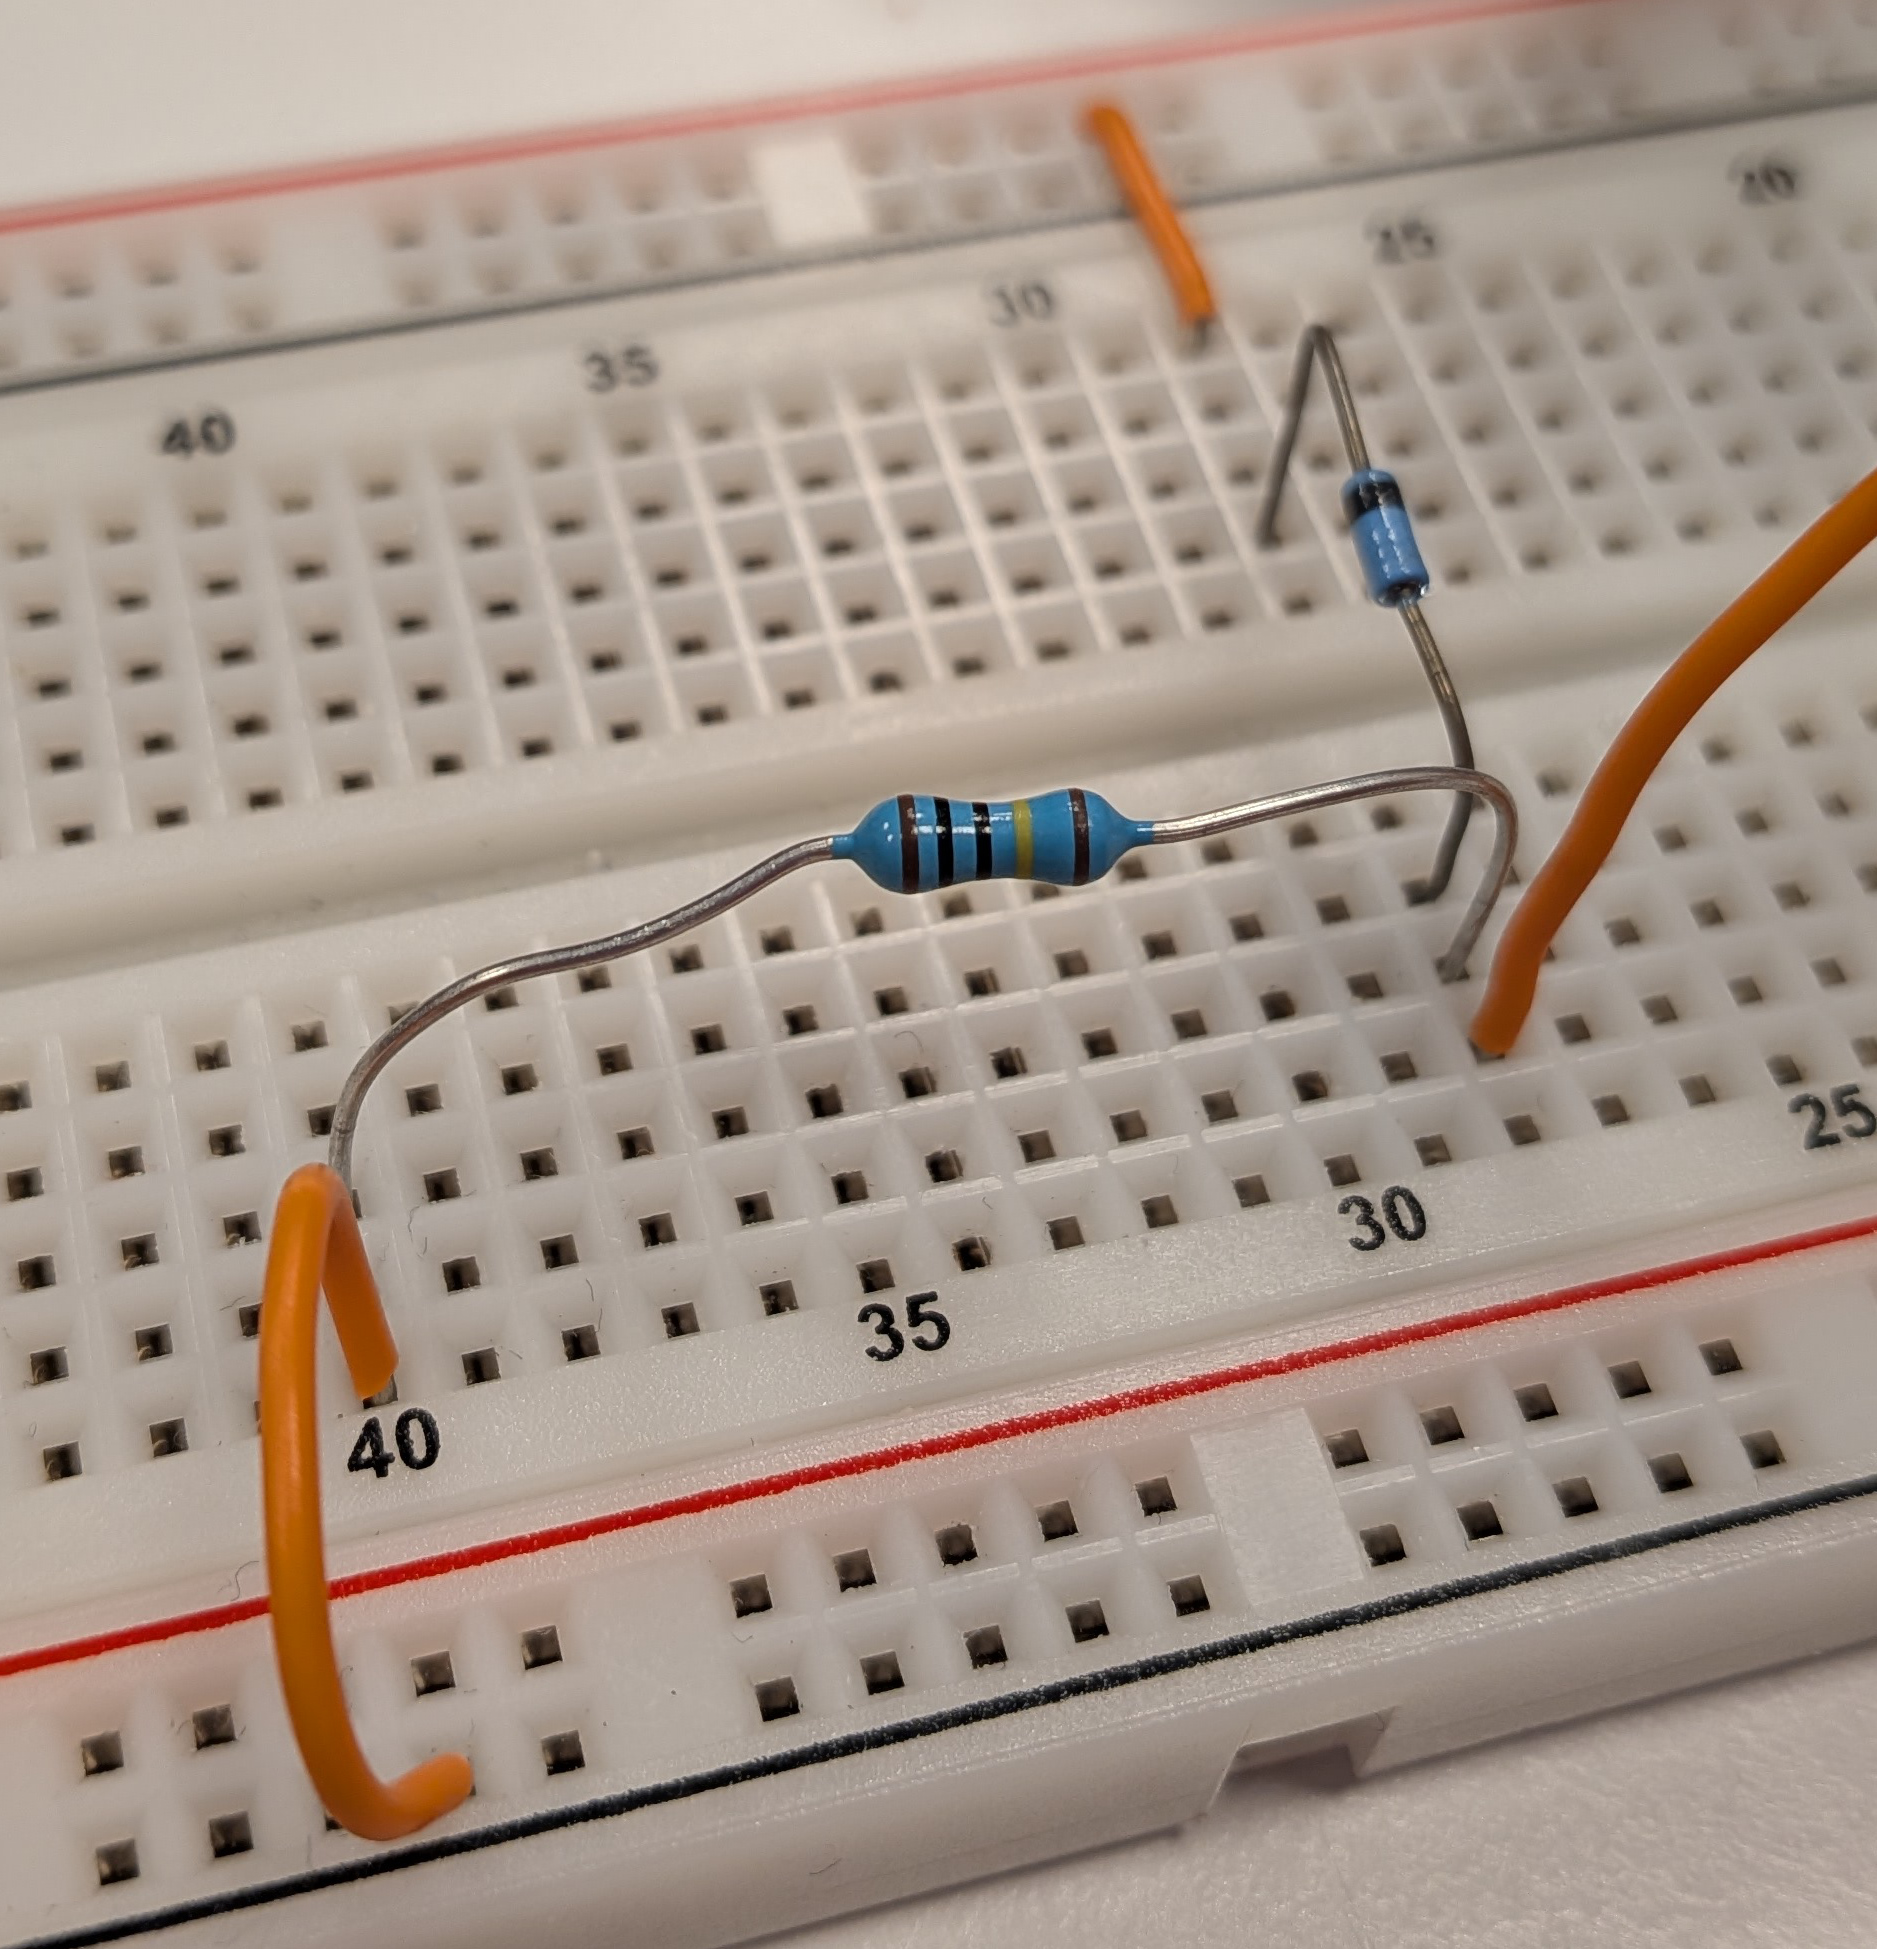
\includegraphics[width=\textwidth]{Part3.jpg}
    \caption{Part 3 circuit}
    \label{fig:Part3}
\end{figure}

\clearpage

%================  TABLE  =========================================================%

% Table generated by Excel2LaTeX from sheet 'Sheet1'
\begin{table}[htbp]
  \centering
  \caption{}
    \begin{tabular}{|l|rl|}
    \hline
    \(E\) (Measured) & 20.03 & V \bigstrut\\
    \hline
    \(R_M\) (Assumed) & 10    & M\Omega \bigstrut\\
    \hline
    \(R\) (Measured) & 1002.5 & k\Omega \bigstrut\\
    \hline
    \(V_R\) (Measured) & 6.2   & mV \bigstrut\\
    \hline
    \(I_S\) (Calculated) & 6.805 & nA \bigstrut\\
    \hline
    \(R_{DC}\) (Calculated) & 2942.71 & M\Omega \bigstrut\\
    \hline
    \end{tabular}%
  \label{tab:Part3}%
\end{table}%

It looks as if the values for \(I_S\) and \(R_{DC}\) miss by an order of magnitude or two as the calculated reverse-bias resistance often leads to values between hunders of \(\SI{}{\kilo\ohm}\) and up to a hundred \(\SI{}{\mega\ohm}\). The inherent inaccuracies in the measurments are probably the cause of this magnitudinal error.

%================  SECTION  =======================================================%

\section{Part 4 - LED charachteristics}
This part is about testing the charachteristics of LED's.

%================  SINGLE FIGURE  =================================================%

\begin{figure}[h]
    \centering
    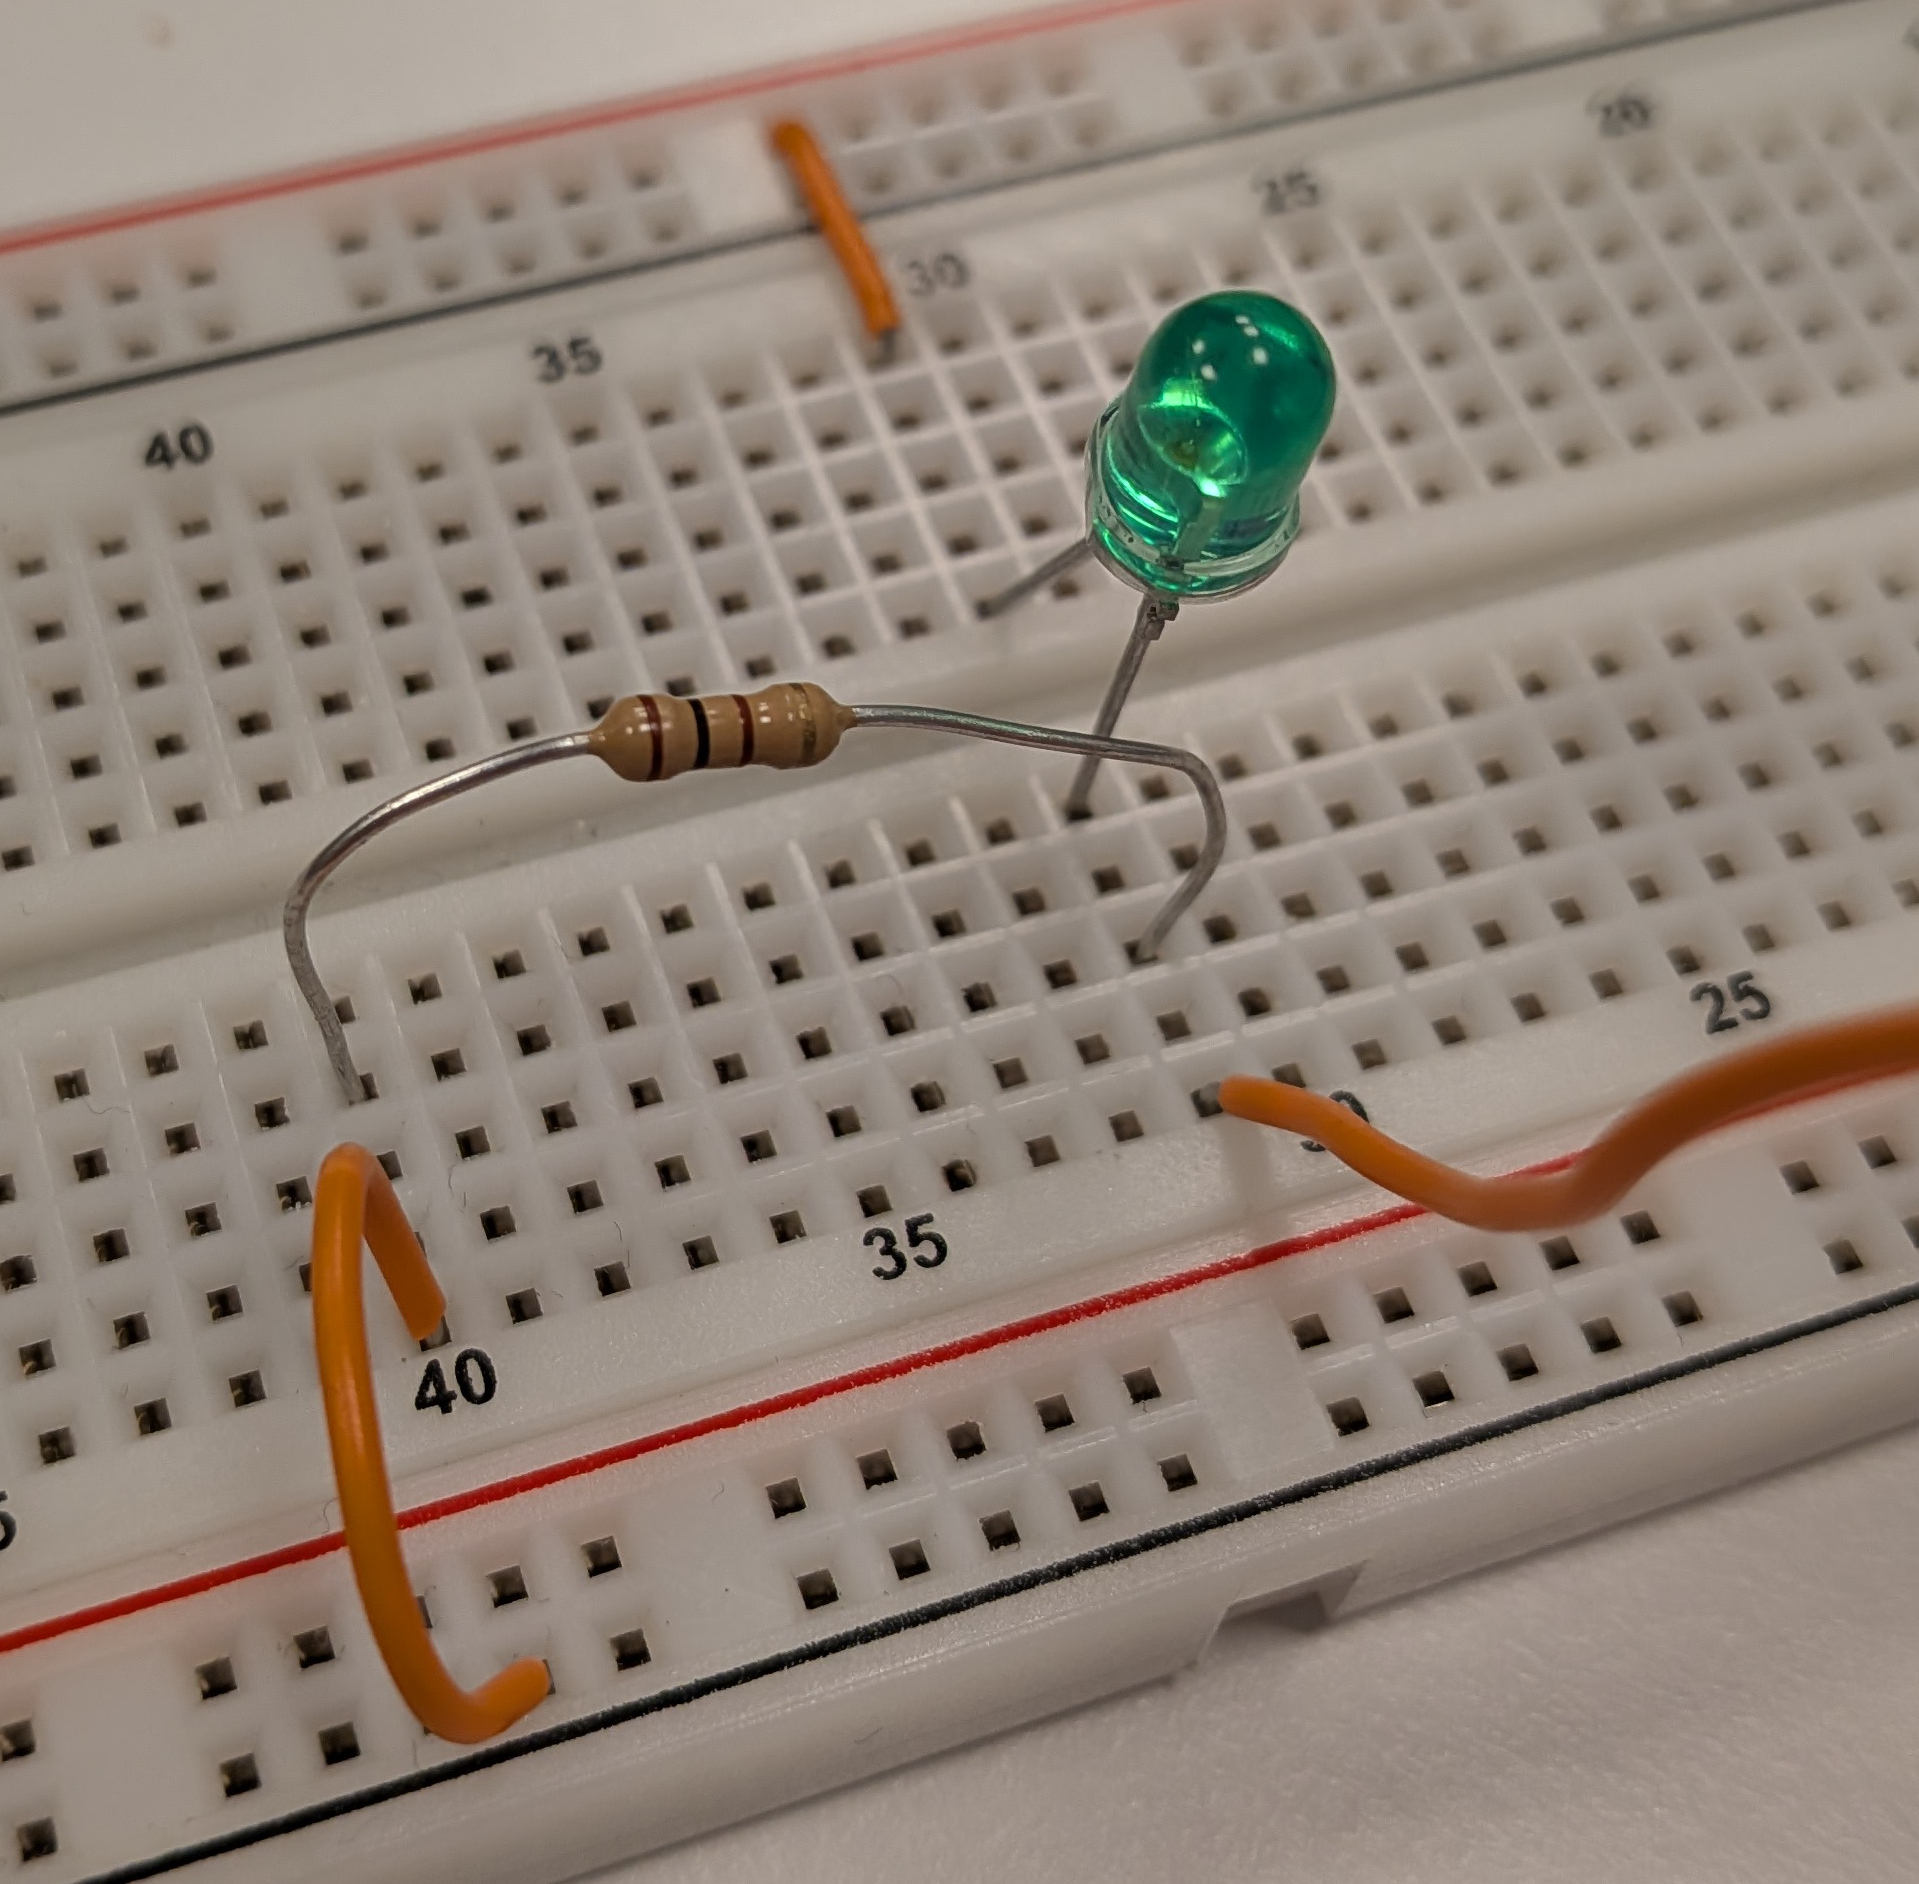
\includegraphics[width=\textwidth]{Part4.jpg}
    \caption{Part 4 circuit}
    \label{fig:Part4}
\end{figure}

%================  TABLE  =========================================================%

% Table generated by Excel2LaTeX from sheet 'Sheet1'
\begin{table}[htbp]
  \centering
  \caption{}
    \begin{tabular}{|l|rl|rl|}
    \hline
    Measurments & \multicolumn{2}{c|}{First light} & \multicolumn{2}{c|}{Bright} \bigstrut\\
    \hline
    \(V_D\) (Measured)   & 1.787   & V   & 2.185  & V \bigstrut\\
    \hline
    \(V_R\) (Measured)   & 17.8    & mV  & 3.632  & V \bigstrut\\
    \hline
    \(I_D\) (Calculated) & 179.980 & μA  & 36.724 & mA \bigstrut\\
    \hline
    \end{tabular}%
  \label{tab:part4}%
\end{table}%

\clearpage

%================  MULTI-FIGURE (WITH SUBFIGURES)  ================================%


\begin{figure}[h]
    \centering
    \begin{subfigure}[t]{0.49\textwidth}
        \centering
        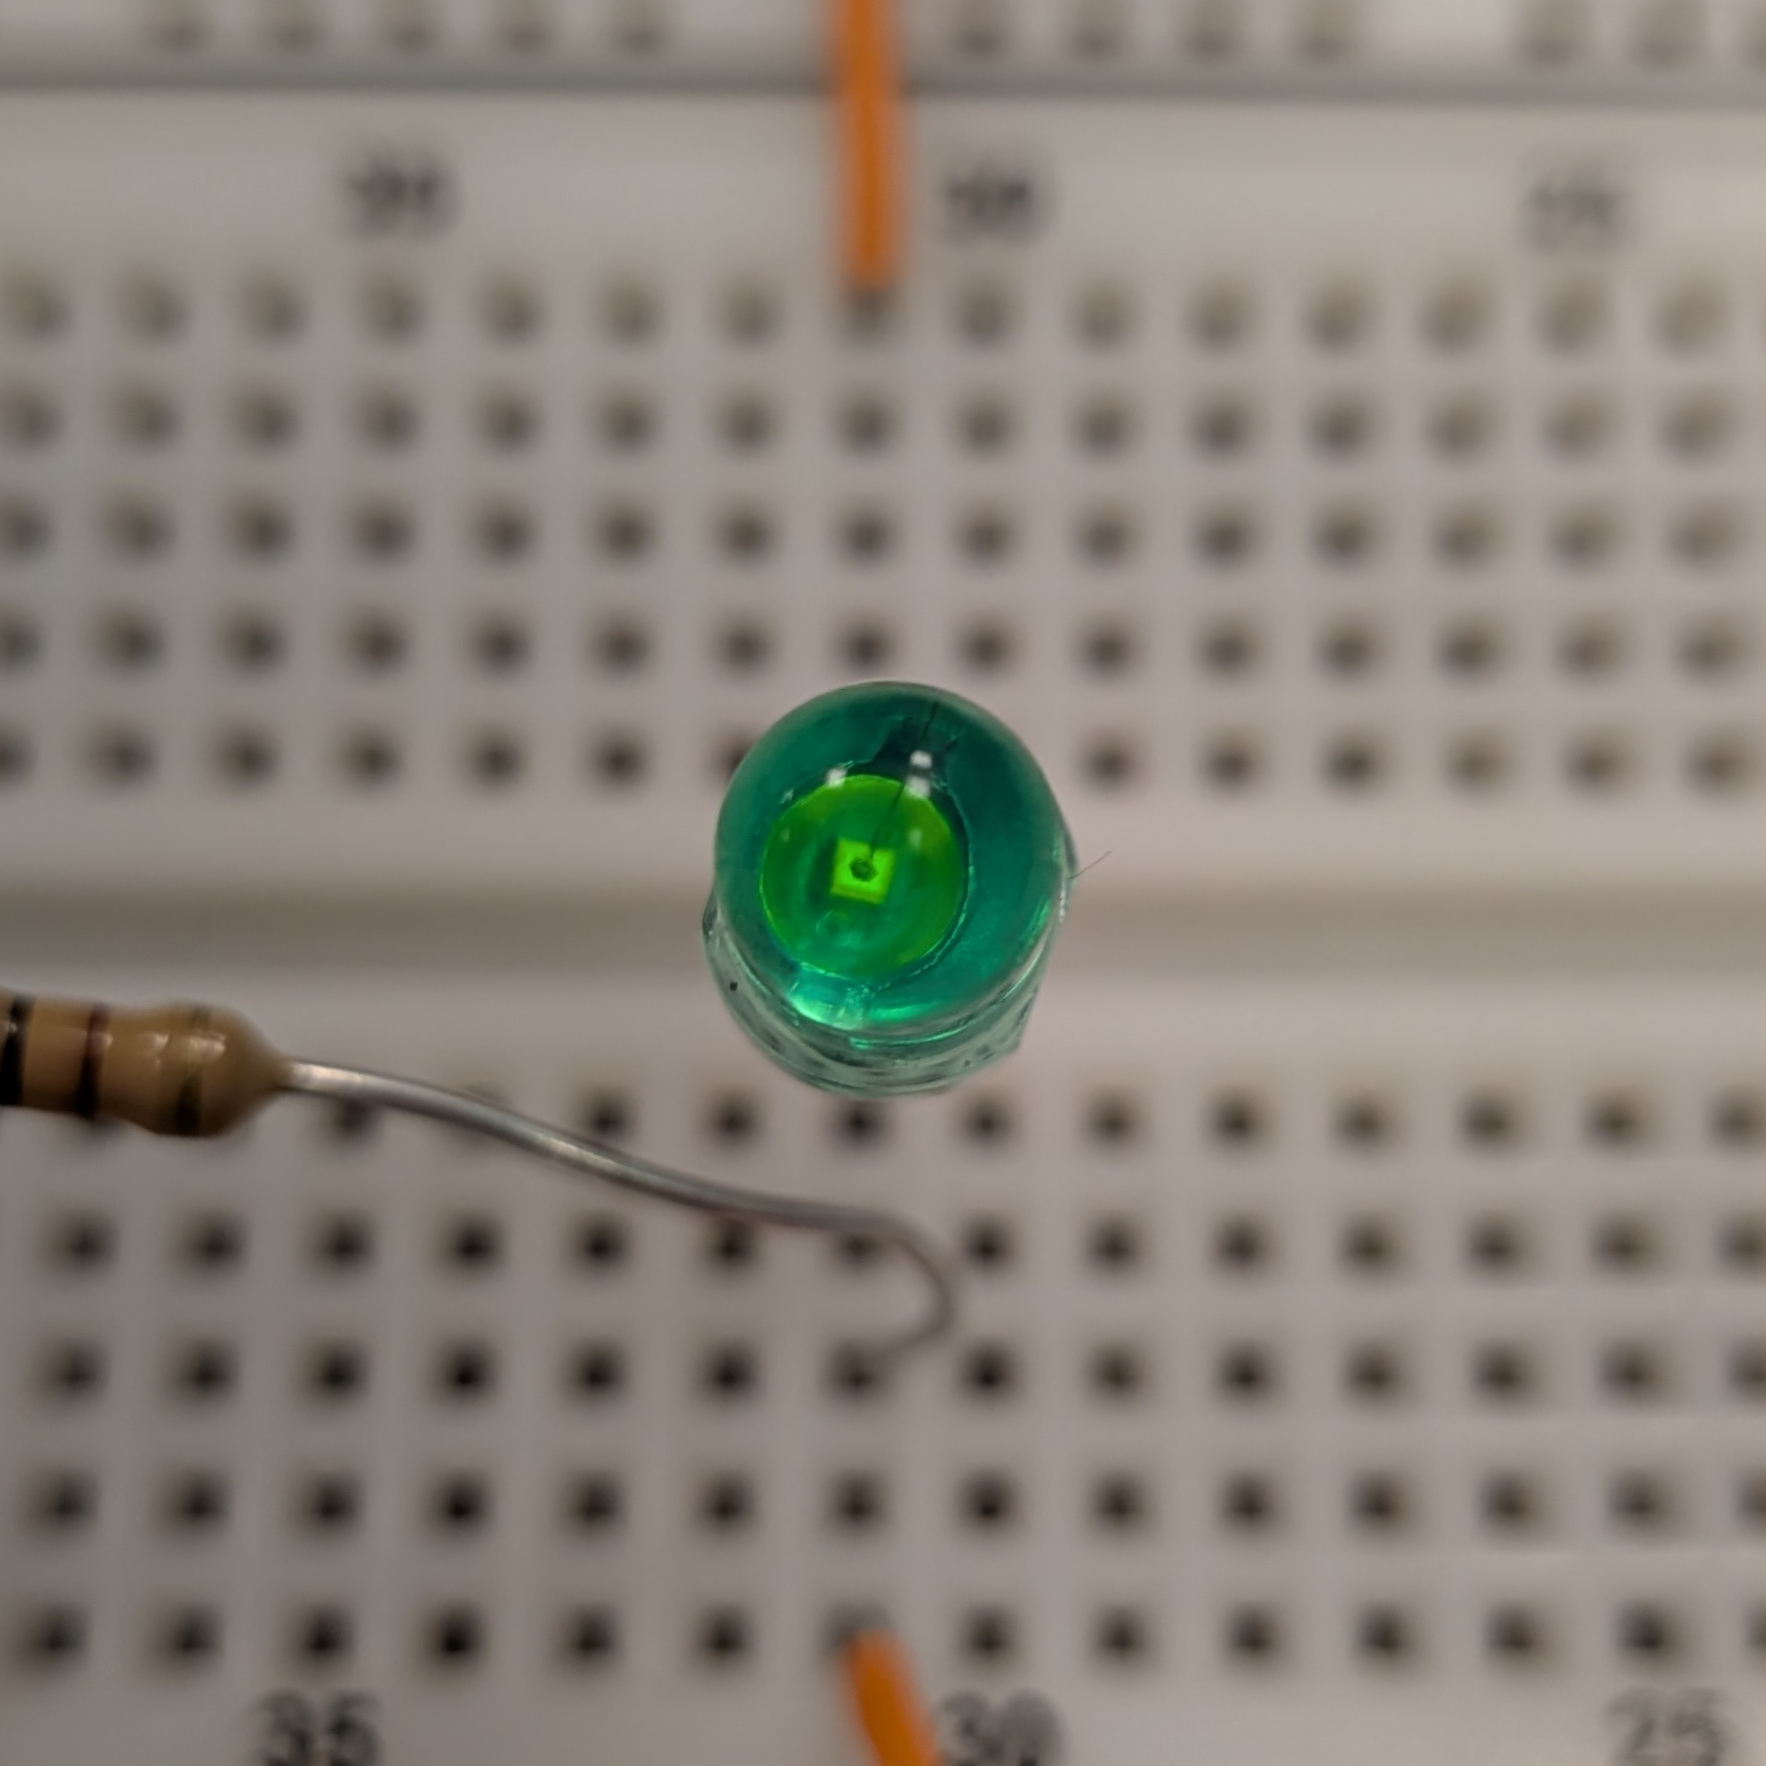
\includegraphics[width=0.9\textwidth]{Part4_FirstLight.jpg}
        \subcaption{First light}
    \end{subfigure}
    \hfill
    \begin{subfigure}[t]{0.49\textwidth}
        \centering
        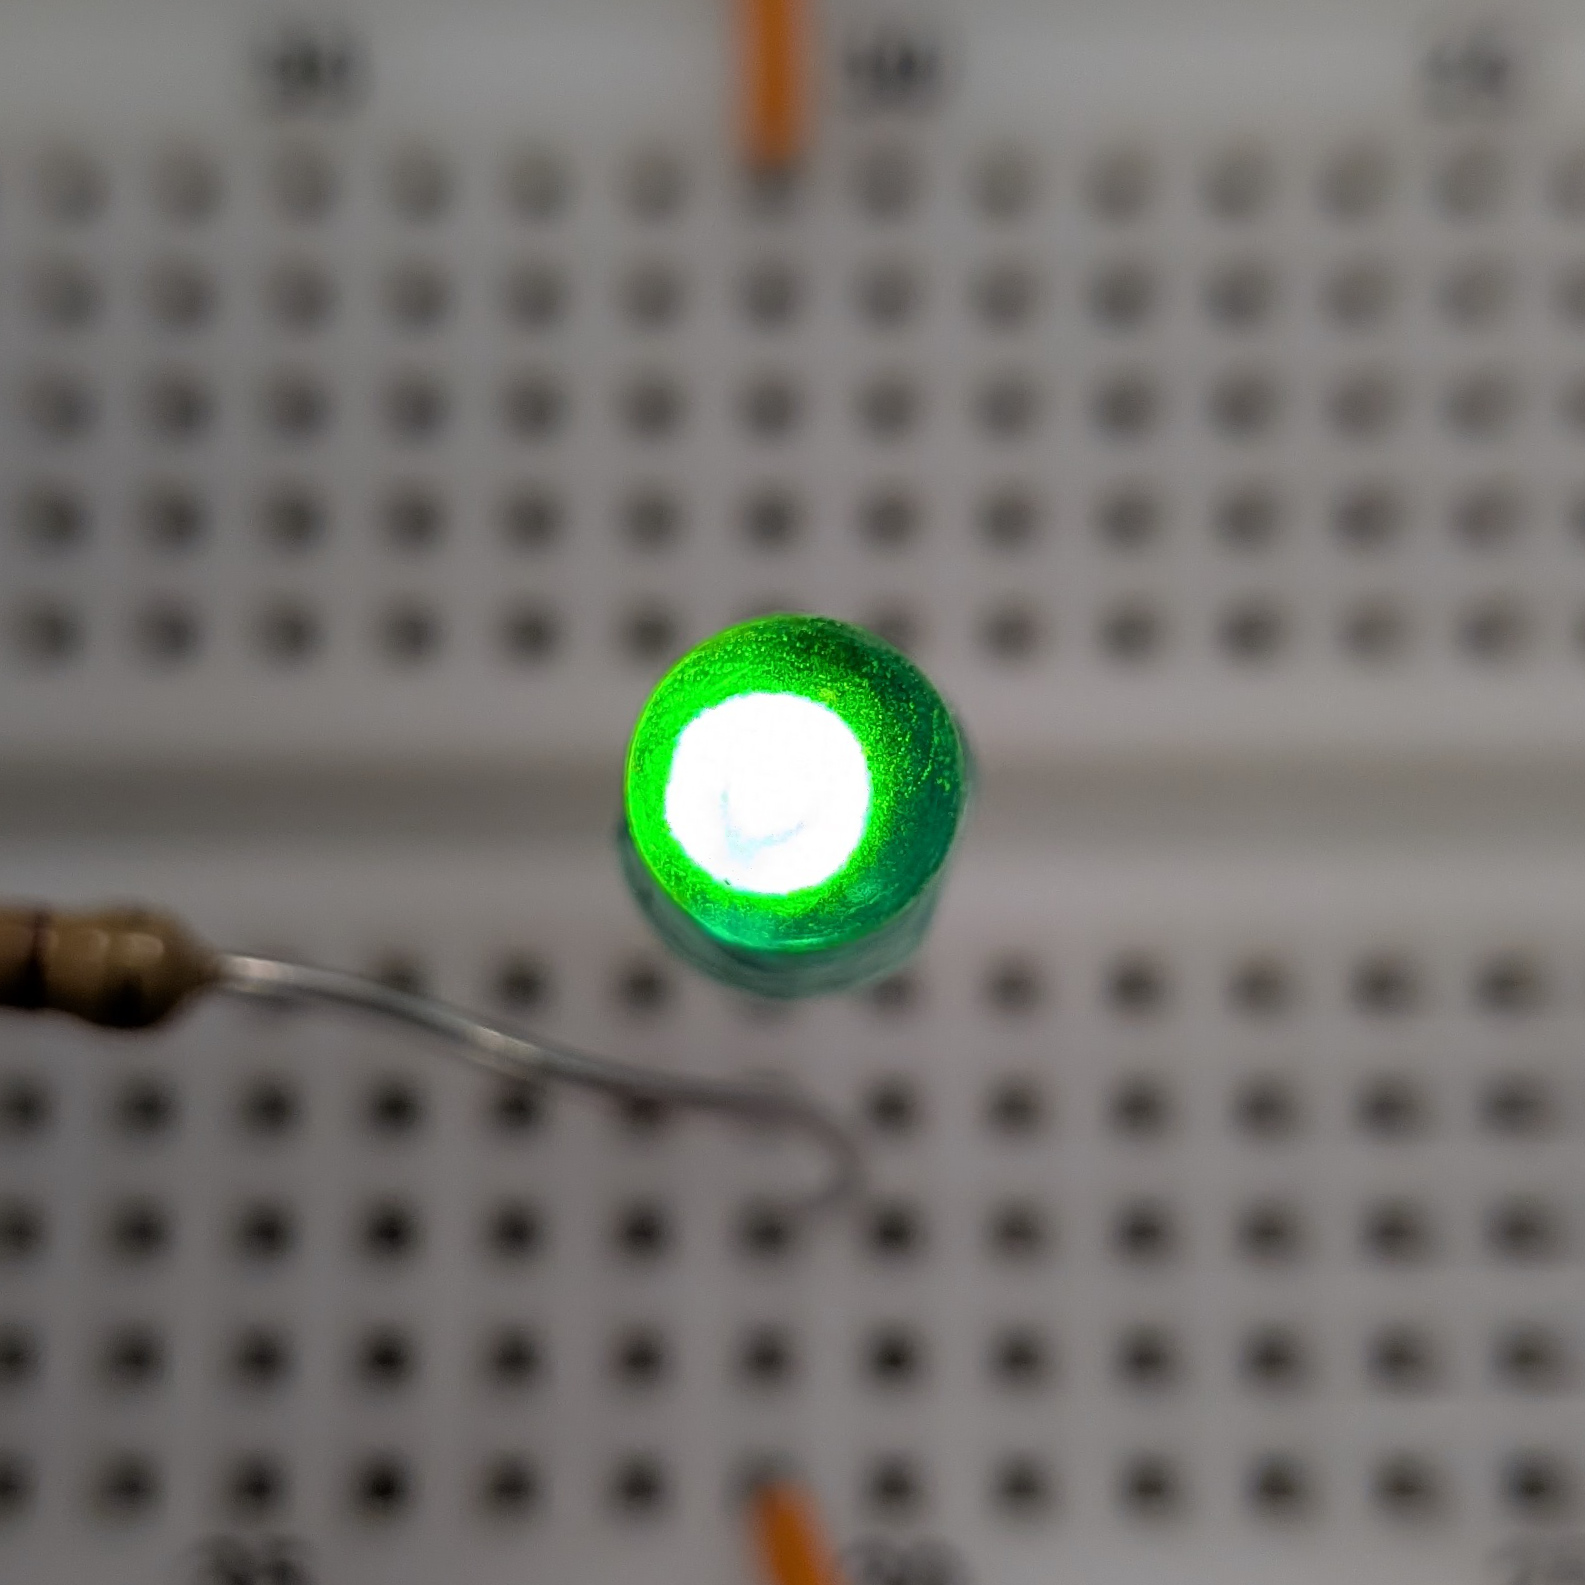
\includegraphics[width=0.9\textwidth]{Part4_FullyOn.jpg}
        \subcaption{Bright}
    \end{subfigure}
    \label{fig:Part4States}
    \caption{Part 4 circuit}
\end{figure}


\end{document}